\section*{Performance analysis}
\subsection*{Theoretical Background}
When it comes to accuracy analysis of a recognizer two classical characteristics are used : The Word error rate, $WER$, and the Accuracy, $Acc$. If we call $N$ the number of words in a sentence, $D$ the number of deletions, $I$ the number of insertions and $S$ the number of substitution, those two characteristic are computed as follow: 
\begin{align*}
WER = \frac{(I + D + S)}{N},\\
Acc = \frac{(N-D-S)}{N}.
\end{align*}
Accuracy doesn't take into account the number of insertions. Therefore, it a worse measure than the WER for most tasks, since insertions are also important in final results. However, for some tasks, accuracy is a reasonable measure of the decoder performance. 

To compute $I$, $D$ and $S$, one may use dynamic programming. The dynamic time warping algorithm that we can use to compute the performance of a recognizer goes as follows:

\begin{algorithm}[H]
 \KwData{Two sentences the true one (size $N$) and the recognize one (size $N'$)}
 \KwResult{Distance between the sentences}
 \For{i=1 to $N'$}{
  \For{j=1 to $N$}{
  AccD[i,j] = LocD[i,j] + min(AccD[i-1,j], AccD[i-1,j-1], AccD[i,j-1])
  }
 }
\caption{Dynamic Time Warping Algorithm}
\end{algorithm}

In the algorithm, $LocD[i,j]$ represents the distance between word number $i$ in the first sentence and word number $j$ in the second one. Here, we take  $LocD[i,j] = 0$ if the two words are the same and $LocD[i,j] = 1$ if they are different. $AccD[i,j]$ represent the shortest possible accumulate distance between the first sentence up to the $ith$ word and the second sentence up the $jth$ word. 

To access the path so as compute $I$, $D$ and $S$, one use backtracking, i.e one remember the paths followed to get the minimum. Figure \ref{fig:dyn_prog} illustrates how the overall algorithm works for comparing two words (and not two sentences). The matrix in the background is the matrix $AccD$.

\begin{figure}[h!]
\center{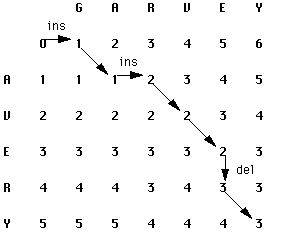
\includegraphics[width=0.4\linewidth]{dyn_prog.png}}
\caption{Dynamic Programming. \cite{dyn_prog}}
\label{fig:dyn_prog}
\end{figure}

\subsection*{One word grammar}
In the game, our grammar is very basic. It consist of sentences of only one word. The possible words are the eight colors : Black, Blue, Pink, Green, White, Orange, Yellow, Red. Our first task was to analyze the accuracy of the model for the framework of our game. 

The results of our tests were very clear. In a quiet environment, we reached 100\% of accuracy. Even the word Black and Blue which have two common phonemes were not confused. Therefore, we decided to do a more advanced performance analysis.

\subsection*{Loop grammar}
A second accuracy analysis was performed using loop grammar. That is a less restricted grammar where a sentence can contain any number of colors. However, the dictionary was not changed. It was still composed of the eight colors: Black, Blue, Pink, Green, White, Orange, Yellow, Red. 
The analysis was done with 15 sentences of random length between three and six. The test was done on two different speakers. $S_1$ was a male speaker with native language Swedish and $S_2$ a female speaker whose native language was french. 

Tables \ref{tad:david_result} and \ref{tad:clem_result} gather our results. On the tables, lines represent the words really spoken (TR) and columns the recognize words (RW).

One can now compute the WER and Accuracy of the results on our experiment for each speaker and then for both together. 

\begin{align*}
WER(S_1) = \frac{2 + 11 +16}{67} = 0.433, Acc(S_1) = \frac{67-11-16}{67} = 0.597
\end{align*}
\begin{align*}
WER(S_2) = \frac{4 + 0 + 12}{64} = 0.250, Acc(S_2) = \frac{64-0-12}{64} = 0.813 
\end{align*}
\begin{align*}
WER(tot) = \frac{2 + 11 +16 +4 +0 +12}{67+64} = 0.344, Acc(tot) = \frac{67 + 64 -11-16 - 0 -12}{67 + 64} = 0.702 
\end{align*}

On the confusion matrices, it is interesting to notice that the Word "Blue" is often recognized as "Pink" for both speaker. For both speakers, it is even more often confused than well-recognized. Moreover, the confusion appears only in one direction: from Blue to Pink and never from Pink to Blue. This is quite surprising since those two words has no common phoneme but this error seems consistent. However, since this confusion did not appear while using a one word grammar one may think that some co-articulation phenomenon appears here making those two words easy to confuse while spoken between two other words. 

\begin{table}[h!]
  \begin{tabular}{|l|*{8}{c|}}
\hline
 TW/RW  & Black & Blue & Pink & Green & White & Orange & Yellow & Red \\
\hline
Black &	5 & & & & 2 & & &  \\
\hline	
Blue  &	& 4 & 5 & & & & & \\
\hline
Pink  & & & 11 & & & & & \\
\hline					
Green & & & & 5 & & & & \\
\hline
White & & & & & 6 & & & \\
\hline
Orange & & & & & & 1 & 4 & 	\\
\hline
Yellow & & 2 & 1 & & & & 4 & 1 	\\
\hline
Red & & & 1 & & & & & 1 \\
\hline
  \end{tabular}
\caption{Confusion matrix for $S_1$, $I = 2$, $D = 11$, $S=16$}
\label{tad:david_result}
\end{table}

\begin{table}[h!]
  \begin{tabular}{|l|*{8}{c|}}
  \hline
 TW/RW  & Black & Blue & Pink & Green & White & Orange & Yellow & Red \\
\hline
Black & 11 & & & & 1 & & &  \\	
\hline
Blue  &	& 3 & 4 & 1 & & & & \\
\hline
Pink  & & & 8 & & & & & \\
\hline				
Green & & & & 5 & & & & \\
\hline
White & & & & & 8 & & & \\
\hline
Orange & & & & & & 11 &  & 	\\
\hline
Yellow & & & & & & & 5 & \\
\hline
Red & & & 3 & & & 3 & & 1 \\
\hline
  \end{tabular}
\caption{Confusion matrix for $S_2$, $I = 4$, $D = 0$, $S=12$}
\label{tad:clem_result}
\end{table}
